\section{Structs and Trees}
\label{sec:structs}

\subsection{\texttt{struct}}

\code{struct} defines a new kind of compound value. One line
\begin{lstlisting}
(struct bt (label left right) #:transparent)
\end{lstlisting}
generates five functions:
\begin{itemize}
  \item \code{bt}, the constructor: \rkt|(bt 1 empty empty)|;
  \item \code{bt?}, a predicate that answers \code{\#t} for these values;
  \item \code{bt-label}, \code{bt-left}, \code{bt-right}, the accessors for the three fields.
\end{itemize}

\begin{pitfall}[Forgetting \code{\#:transparent}]
Without \code{\#:transparent}, a struct value prints as \code{\#<bt>} with its contents hidden, and \code{equal?} is true only when the two values are the very same object. Two trees that look identical then compare as different, and every test that compares trees fails. With the flag, values print readably and \code{equal?} compares field by field.
\end{pitfall}

\code{struct} does \emph{not} check the types of its fields. \rkt|(bt 1 2 3)| is accepted, even though 2 and 3 are not trees. Nothing goes wrong until some traversal calls \code{bt-label} on the number 2, possibly far from the line that built the bad value. \Cref{sec:definetype} returns to this point: \code{define-type} in \code{plai-typed} rejects such a value where it is built.

\subsection{Binary Trees}

The empty tree is represented by \code{'()}, so a binary tree is either \code{empty} or a \code{bt} with a label and two subtrees.
\begin{lstlisting}
(define tree
  (bt 1
      (bt 2 empty empty)
      (bt 3 empty empty)))
\end{lstlisting}

The definition of a tree mentions trees in \emph{two} places, left and right, so a function over trees has two recursive calls. Lists mentioned themselves once, and list functions had one. The shape of the code follows the shape of the data (\Cref{fig:bt}).

\begin{lstlisting}
(define (sum-bt t)
  (cond
    [(empty? t) 0]
    [(bt? t) (+ (bt-label t)
                (sum-bt (bt-left t))
                (sum-bt (bt-right t)))]
    [else (error 'sum-bt "not a tree: ~a" t)]))
\end{lstlisting}

\begin{figure}[htbp]
\centering
\begin{tikzpicture}[level distance=11mm, sibling distance=24mm,
    every node/.style={ast}, level 2/.style={sibling distance=12mm}]
  \node {bt 1}
    child {node {bt 2} child {node[astl] {'()}} child {node[astl] {'()}}}
    child {node {bt 3} child {node[astl] {'()}} child {node[astl] {'()}}};
\end{tikzpicture}
\hspace{1.2cm}
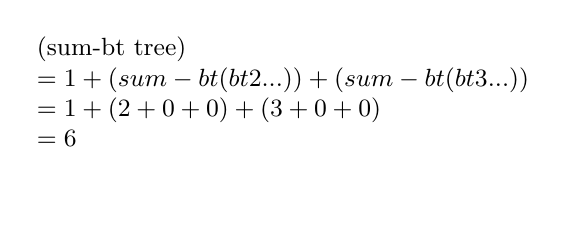
\begin{tikzpicture}[baseline=-14mm]
  \node[draw=none, fill=none, align=left, font=\small] {
    \code{(sum-bt tree)}\\
    $= 1 + \code{(sum-bt (bt 2 ...))} + \code{(sum-bt (bt 3 ...))}$\\
    $= 1 + (2 + 0 + 0) + (3 + 0 + 0)$\\
    $= 6$};
\end{tikzpicture}
\caption{The value \code{tree}. Each \code{bt} node causes two recursive calls, one per subtree.}
\label{fig:bt}
\end{figure}

Tree recursion is usually not made tail-recursive: with two recursive calls, at most one of them can be the last thing the function does, and the other has to be remembered.

\subsection{\texttt{match}}

\code{match} checks the shape and extracts the fields in one step, which reads better once all the fields are needed anyway:
\begin{lstlisting}
(define (sum-bt/match t)
  (match t
    ['() 0]
    [(bt label left right)
     (+ label (sum-bt/match left) (sum-bt/match right))]))
\end{lstlisting}
The pattern \rkt|(bt label left right)| matches only \code{bt} values and binds the three names to the fields in order.

\subsection{(SUPPLEMENT) Further Topics}

\subsubsection{Structural recursion} Functions like \code{sum-bt} are \emph{structurally recursive}: they recur only on immediate sub-parts of their input. Such functions always terminate on finite data, since each call is on a strictly smaller value, and their correctness can be proved by \emph{structural induction}, one case per variant. Every interpreter in this course is structurally recursive in its \code{eval} on the abstract syntax tree, except where substitution builds a new tree (\Cref{ch:week4}).

\subsubsection{Opaque structs and abstraction} Opacity is the default for a reason: an opaque struct hides its representation, so a module can export the struct without letting clients inspect or compare its insides. Transparent structs are the right choice for plain data such as trees and syntax, where structural equality is what you want. A middle ground is \code{\#:prefab}, which also makes structs readable and writable as literals.

\subsubsection{Contracts on fields} Plain Racket can check field types at run time with \code{struct/contract} or \code{contract-out}, e.g.\ requiring \code{left} to satisfy \code{(or/c empty? bt?)}. The error then points at the bad construction rather than the later traversal. \code{plai-typed} (\Cref{ch:week3}) instead checks before the program runs.
